\documentclass[10pt,xcolor={dvipsnames}]{beamer}
\usetheme{Antibes}
\usepackage[utf8]{vietnam}
\usepackage{graphicx}

\title{Google Trace Data Streaming System}
\author{Nhóm 1}

\begin{document}
	\begin{frame}
		\maketitle
	\end{frame}
	
	\begin{frame}
		\tableofcontents
	\end{frame}
	
	\section{Giới thiệu bài toán}
	
	\begin{frame}{Giới thiệu}
		\begin{block}
		{Bài toán thực tế}
		Thực hiện mô phỏng hệ thống theo dõi trạng thái cuả một trung tâm máy chủ và quản lý hoạt động của các máy tính trong trung tâm máy chủ.
		\end{block}
		
		\begin{block}
		{Mô hình hoạt động thực tế}
		\begin{figure}
			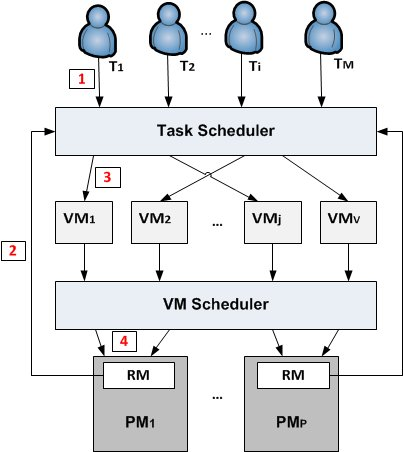
\includegraphics[scale=0.25]{images/Task-and-VM-scheduling-in-cloud-computing_W640.jpg}
		\end{figure}
		\end{block}
	\end{frame}
	
	\section{Đặc điểm dữ liệu}
	
	\begin{frame}
	{Dữ liệu mô phỏng} 
	\begin{block}
	{Nguồn}
	Là các file csv google publish, phiên bản đầu tiên vào ngày 27/10/2011
	\end{block}
	\begin{block}
	{Đặc điểm}
	Gồm 6 loại dữ liệu: 
	\begin{itemize}
		\item \textbf{job-event}: lưu lại các thông tin job được submit 
		\item \textbf{machine-attributes}: chứa thông tin của các máy tính trong trung tâm máy chủ 
		\item \textbf{machine-events}: chứa thông tin cấu hình của các máy tính trong trung tâm máy chủ 
		\item \textbf{task-event}: chứa thông tin các task được submit 
		\item \textbf{task-constraints}: chứa các điều kiện rằng buộc của các task
		\item \textbf{task-usage}: chứa thông tin trong thời gian thực thi các task 
	\end{itemize}
	\end{block}
	\end{frame}
	
	\begin{frame}
		\begin{block}
		{Số lượng máy tính} 12583
		\end{block}
		\begin{block}
		{Phân phối cấu hình}
		\begin{figure}
			\centering
			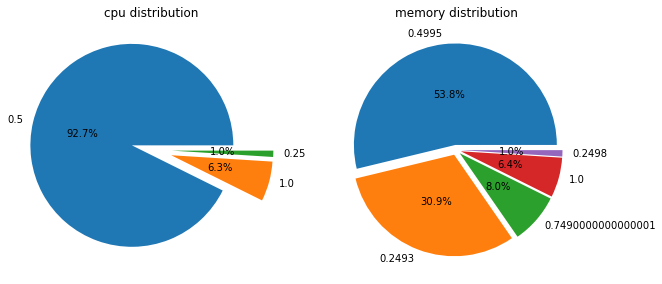
\includegraphics[scale=0.35]{images/machine_attributes.png}
		\end{figure}
		\end{block}
	\end{frame}
	
	\begin{frame}
	{Thông tin task được submit}
	\begin{figure}
		\centering
		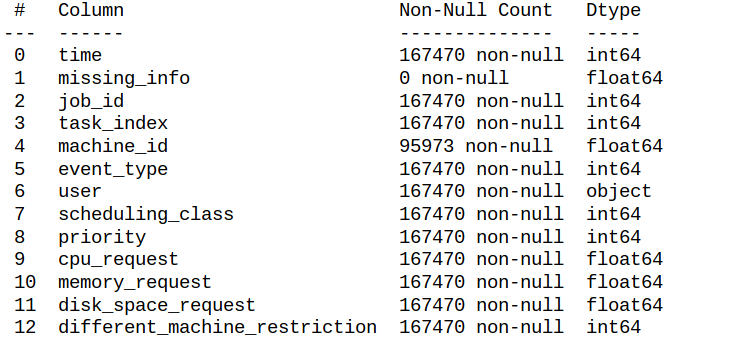
\includegraphics[scale=0.5]{images/task_event_schema.png}
	\end{figure}
	\end{frame}
	
	\begin{frame}
	{Thông tin task được submit}
	\begin{block}
	{Số lượng task đến hệ thống trong 1 giây}
	\begin{figure}
		\centering
		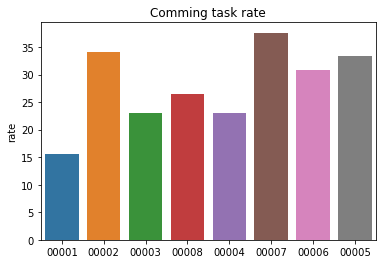
\includegraphics[scale=0.45]{images/comming_task_rate.png}
	\end{figure}
	\end{block}
	
	\begin{block}
	{Trung bình}
	28 tasks / 1 giấy được gửi đến hệ thống
	\end{block}
	\end{frame}
	
	\section{Mô hình hệ thống}
	
	\begin{frame}
	{Mô hình giải quyết bài toán}
		\begin{block}
			{Mục tiêu}
			Xây dựng mô hình theo dõi được lượng task đang đến hệ thống và thực hiện phân tích, đánh giá và lưu trữ theo thời gian thực. 
		\end{block}
		\begin{block}
		{Mô hình}
		\begin{figure}
			\centering
			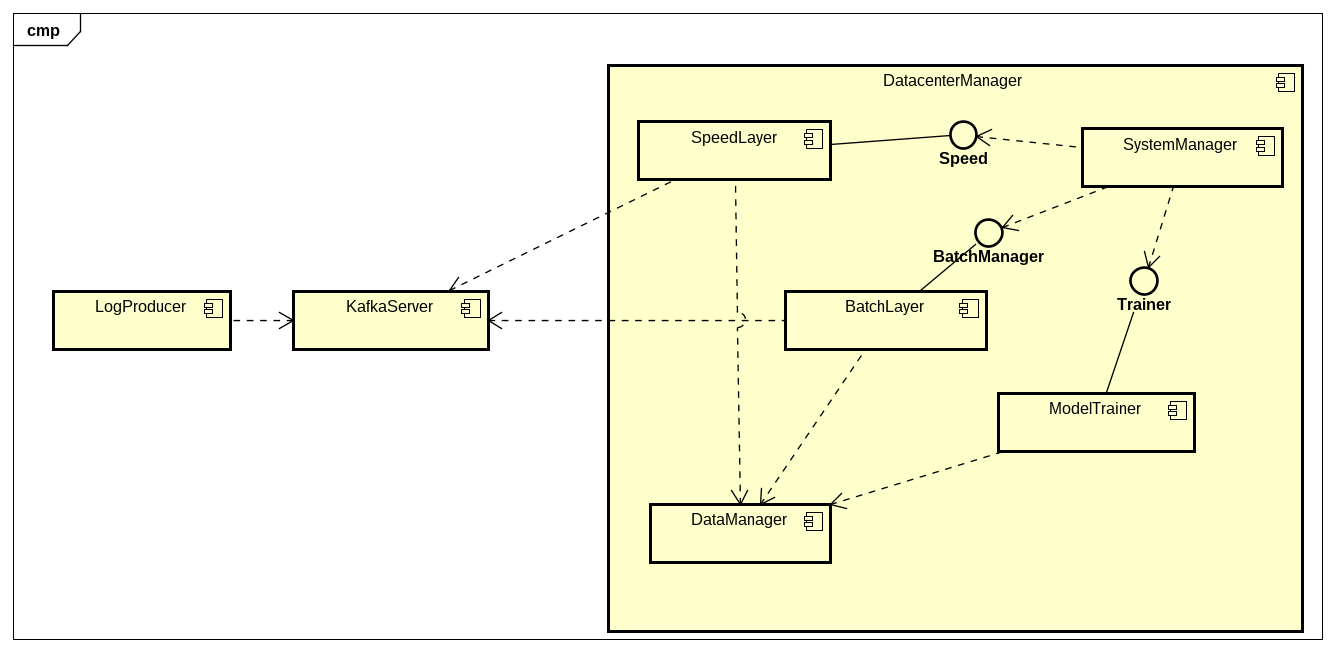
\includegraphics[scale=0.25]{images/LogStreamingComponents.png}
		\end{figure}
		\end{block}
	\end{frame}	
	
	\begin{frame}
	{Các thành phần cài đặt}
	\begin{figure}
		\centering
		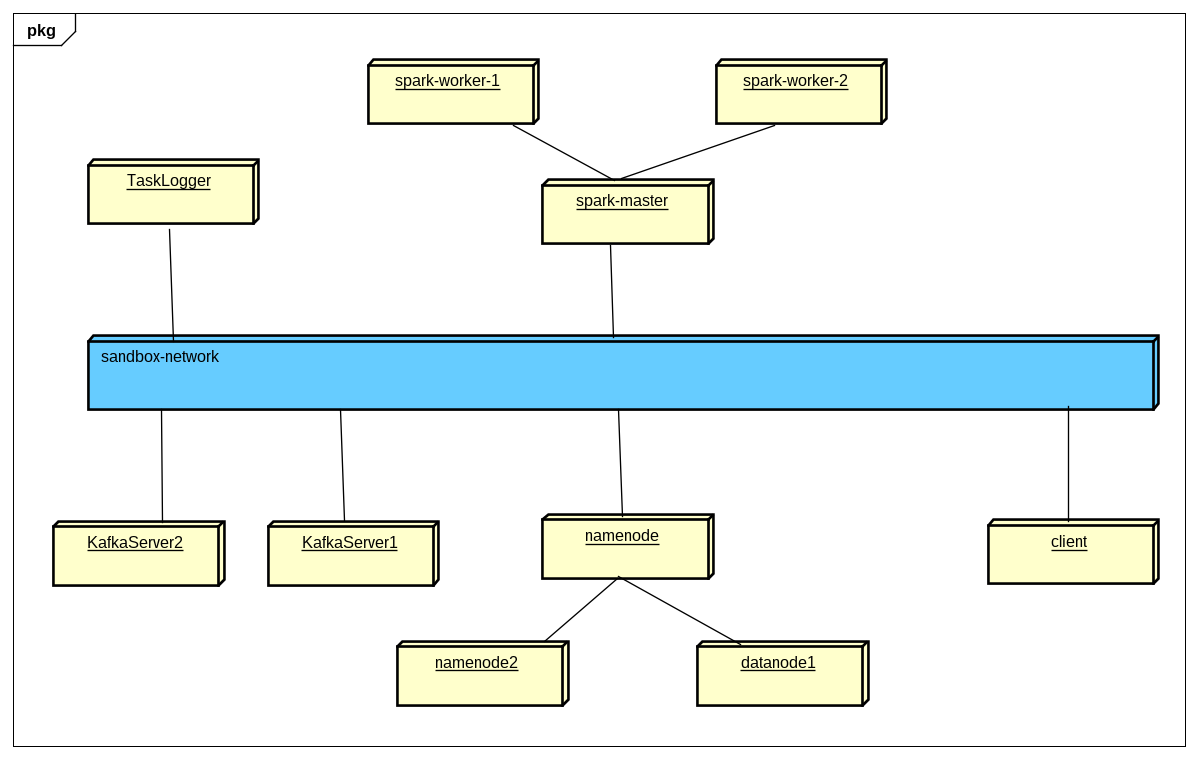
\includegraphics[scale=0.25]{images/DeploymentDiagram.png}
	\end{figure}
	\end{frame}
	
	\section{Batch Layer - Xây dựng mô hình học máy}
	
	\begin{frame}
	{Tại sao sử dụng mô hình học máy}
	\begin{block}
	{Đặc điểm của các máy tính trong hệ thống}
	Hệ thống gồm rất nhiều máy tính được phân chia vào các cấu hình khác nhau, do đó các task đến hệ thống cần được phân chia vào các nhóm có cấu hình phù hợp. 
	\end{block}
	
	\begin{block}
	{Đặc điểm của các task}
	Từng task sẽ có yêu cầu tài nguyên khác nhau, nên sẽ được chia vào các nhóm máy tính khác nhau. 
	\end{block}
	
	\begin{block}
	{Giảm thời gian lập lịch}
	Thay vì tìm một máy tính thích hợp cho một task trên toàn bộ máy tính, ta chia các máy tính thành từ nhóm, phân task vào một nhóm và thực hiện thuật toán lập lịch trên số lượng máy tính nhỏ hơn.
	\end{block}
	\end{frame}
	
	\begin{frame}
	{Mô hình phân cụm task}
	\begin{block}{Phân cụm}
		\begin{figure}
			\centering
			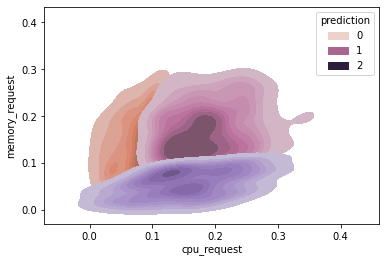
\includegraphics[scale=0.35]{images/task_cluster.png}
		\end{figure}
	\end{block}

	\begin{block}
	{Kết quả}
	\begin{itemize}
		\item $memory\_request < 0.1$
		\item $cpu\_request < 0.1$ và $memory\_request \geq 0.1$
		\item $cpu\_request \geq 0.1$ và $memory\_request \geq 0.1$
	\end{itemize}
	\end{block}		
	
	\end{frame}
	
	\section{Speech Layer - Phân tích dữ liệu thời gian thực} 
	
	\begin{frame}
	{Các công việc monitor}
		\begin{block}
		{Xử lý dữ liệu}
		\begin{itemize}
			\item Nhận dữ liệu từ broker
			\item Extract các thông tin cần thiết
		\end{itemize}
		\end{block}
		
		\begin{block}
		{Trung bình các thông số}
		\begin{itemize}
			\item cpu request
			\item memory request
			\item cpu request per machine
			\item memory request per machine
		\end{itemize}
		\end{block}
	\end{frame}
	
	\section{Kiểm thử hiệu năng hệ thống}
	
	\begin{frame}
	{Spark}
		\begin{block}
		{Train clustering model (spark-worker config: 1 core 1g ram)}
		\begin{itemize}
			\item 2 worker 4 partitions: 27.3 s 
			\item 1 worker 2 partitions: 22.8 s
			\item 0 worker: Lost
		\end{itemize}
		Do đặc điểm của môi trường mô phỏng cụm phân tán nên có thể dẫn đến việc train mô hình với 2 worker chậm hơn so với 1 worker.
		\end{block}
	\end{frame}
	
	\begin{frame}
	{Kafka}
	\end{frame}
	
\end{document} 
